\documentclass{standalone}
\usepackage{standalone}

\usepackage{tabularx}
\begin{document}
\newcolumntype{L}[1]{>{\raggedright\arraybackslash}p{#1}}
\newcolumntype{C}[1]{>{\centering\arraybackslash}p{#1}}
\newcolumntype{R}[1]{>{\raggedleft\arraybackslash}p{#1}}

\chapter{Background Study}
Background study is one of the important preliminary steps for any thesis work. Studying the related works of literature and relevant works help us to initiate our work in a systematic way. That can be described below. Actually, our background study introduces how to process an acoustic signal or voice and to build an Acoustic Model(AM) \cite{mohamed2012acoustic}.

\section{Literature Review}
There is a lot of research work on Speech recognition System. Speech recognition dramatically advances afterward in 1976 as technology made significant development \cite{huang2014historical}. A good literature review helps researchers to find articles related to their topic and should be done for saving time.
\\
Most of the researches of speech recognition are done for English and then Mandarin.
There is only a few research is done for Bangla Language.        
\subsection{ASR in Bangla}
There are few types of research are done on STT for Bangla.
\\
Actually, there are a few research works on the isolated and continuous corpus of Bangla like \cite{das2011bengali, sultana2012bangla, shrishrimal2012indian, rahman2003continuous, huang2014historical, sinha2014speech, islam2009research, hasnat2007isolated, lee1988automatic, karim2002recognition, juang2005automatic}.
A group of people from KUET named Shahena Sultana, Prodip Kumar Das, M. M. Hafizur Rahman of International Islamic University Malaysia worked on Continuous Bangla speech recognition. Their vocabulary size was 270 Bangla words. And they used Application Programming Interface (API) of Microsoft Corporation. Their recognition accuracy rate is 74.81\% \cite{sultana2012bangla}. Md. Ali Hossain, Md. Mizanur Rahman Uzzal Pradhan and Md. Faruquzzaman khan implemented Back Propagation Neural Network for recognizing just Bangla digits. Their performance for the known speaker is 96.33\% and for an unknown speaker, that rate degrades to 92\% \cite{hossain2013implementation}. Md. Abul Hasnat, Jabir Mowla and Mumit Khan of BRAC University did a fantastic research on Isolated and Continuous Bangla Speech Recognition. They apply  HMM-based classifiers. They use distinct 100 Bangla words. For isolated word and speaker dependent and speaker independent rate of recognition respectively are 90\% and 70\% \cite{hasnat2007isolated}. Determining uninterrupted speech with Artificial Neural Network classifier has the average performance rate of 73\% \cite{rahman2003continuous}. Besides, automatic recognition of real numbers was implemented in SUST by Md. Mahadi
Hasan Nahid and Md. Ashraful Islam using CMU SPHINX. And they got 85\% accuracy for personal computer and 75\% accuracy for android mobile \cite{nahid2016noble}. Moreover, M. J. Rahman Saurav and Md. Shakhawat Amin also worked in ASR in SUST for Pipilika as the last previous work. They worked in 500 unique isolated words and took 50 speaker's utterances of those words. And their accuracy was 92\%.
A comparison between these researches is given below \cite{sultana2012bangla}\cite{hossain2013implementation}\cite{hasnat2007isolated}\cite{rahman2003continuous}\cite{nahid2016noble}.
\\
\\
%%% Table starts here:
\begin{table}[ht]
\centering
\begin{tabular}{|C{6cm} | c | c | c|}
\hline 
Topic & Unique Words & Number of Speakers & Average Accuracy \\ [0.8ex] % inserts table column name
\hline % inserts single horizontal line
Bangla Speech -to Text
Conversion using API & 270 & Unknown & 74.81\% \\ 
\hline Implementation of Back Propagation
Neural Network for Isolated
Bangla Speech Recognition & 10 & 10 & 94.17\% \\ 
\hline Isolated and continuous bangla
speech recognition: Implementation
performance and application perspective & 100 & 5 & 75\% \\
\hline A Noble Approach for Recognizing
Bangla Real Number Automatically
Using CMU Sphinx4 & 115 & 15 & 85\% \\
\hline Continuous Bangla Speech
Recognition System & 100 & 5 & 73\% \\
\hline Building an automatic speech recognition system for pipilika voice search in bangla language & 500 & 50 & 92\% \\ [1ex] % [1ex] adds vertical space
\hline %inserts single line

\end{tabular}
\caption{Comparison between various research works on bangla speech recognition} % title of Table
\label{table: comp_researches} % is used to refer this table in the text
\end{table}

\subsection{To know about Kaldi}
Kaldi is an FST based speech recognition framework \cite{povey2011kaldi}. Its code is in the shell script. So, we learned shell script to understand the library of Kaldi. It has an organized folder structure. So we have understood easily about related all folders that means which folder stores which shell script and python files. 

\section{Speech recognizer}
Almost 30 years ago the methods of continuous speech recognition were established. Among all the methods, Hidden Markov Model(HMM) is a one of the most popular statistical method. And we get an open-source toolkit kaldi \cite{povey2011kaldi} for speech related tasks or researches and it is FST based framework that uses this HMM technique. The principals of speech recognition and present techniques are also described in this chapter. Kaldi speech recognizer structure is showed below.
\\
%% For figure drawing ..
\begin{figure}[h]
 \centering
 \centerline{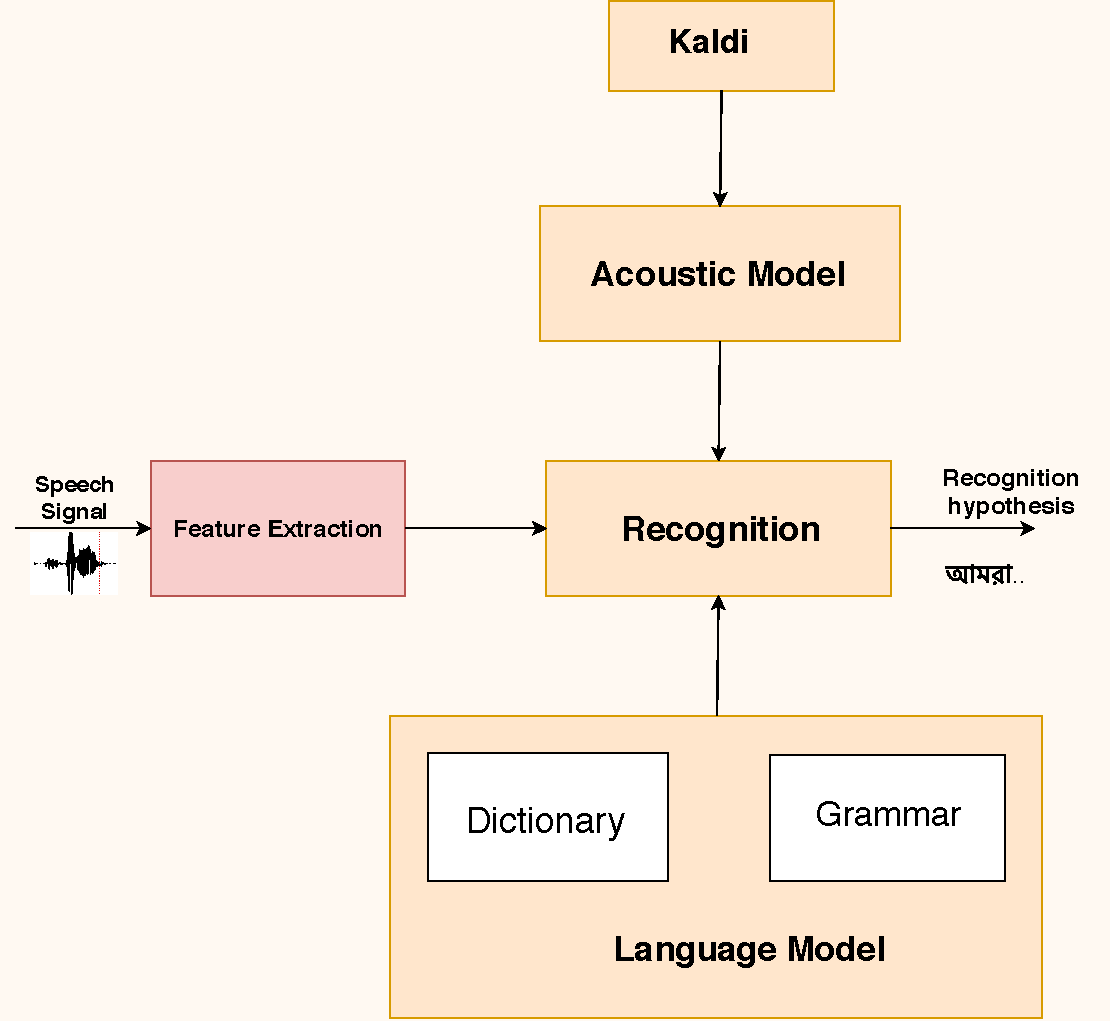
\includegraphics[width=13cm, height=10.5cm]{img/SR_structure.pdf}}
 \caption{Speech recognizer structure}
\label{fig:student}
\end{figure}

In speech recognition, recognizing the word sequence from the speech is equivalent to automatic speech recognition. In Equation \ref{notdependent}, the most probable sequence of words $w*$ given the acoustic observation \cite{lee1988automatic} a formally

    \begin{equation}\label{notdependent}
        w^*=argmax_w{P(w|a)}=argmax_w{\frac{P(a|w)*P(w)}{P(a)}}=argmax_w{P(a|w)*P(w)}
    \end{equation}
    
Here the probability of the acoustic features does not keep changes in the equation. So this can be eliminated.

\subsection{Acoustic modeling}
An acoustic model is a file that contains statistical representations of each of the different sounds that creates a word. A large database of speech makes an acoustic model using these representations. The phoneme is represented at each of these statistical representations. To implement special training algorithms to develop statistical representations for each phoneme in a language which is called Hidden Markov Models(HMMs). Evey phonemes have its individual HMM \cite{boruah2013study}. Also, we have got another type of acoustic model called DBN-DNN \cite{mohamed2012acoustic, hinton2012deep}.

\subsection{Hidden Markov Model}
In the late 1970s and early 1980s, the field of Automatic Speech Recognition (ASR) was undergoing a change in emphasis: from simple pattern recognition methods, based on templates and a spectral distance measure, to a statistical method for speech processing, based on the Hidden Markov Model (HMM) \cite{rabiner1989tutorial, boruah2013study}. Actually, Hidden Markov models are probabilistic frameworks where the observed data are modeled as a series of outputs generated by one of several (hidden) internal states. The model then uses inference algorithms to estimate the probability of each state along with every position along the observed data. That works based on FST. Mono-phones and Tri-phones are the hidden states in term of automatic speech recognition and samples of the acoustic features are observed. Maximum-likelihood estimation for Markov chain and there have the speech recognition process of hybrid HMM and neural net \cite{juang1985maximum, kundu1998speech}.
\\
There are two types of parameters in the Hidden Markov Model such as transition probabilities among states and probabilistic distribution for generating observation in a given state. The training of the Acoustic Model evaluates these parameters. There is also a DNN model with HMM.\\

In HMMs, the parameter learning finds the best set of state transition and emission probabilities from a given output sequence. An HMM is able to model variable length of phones. A DNN based HMM structure is shown below.\\


\begin{figure}[h]
 \centering
 \centerline{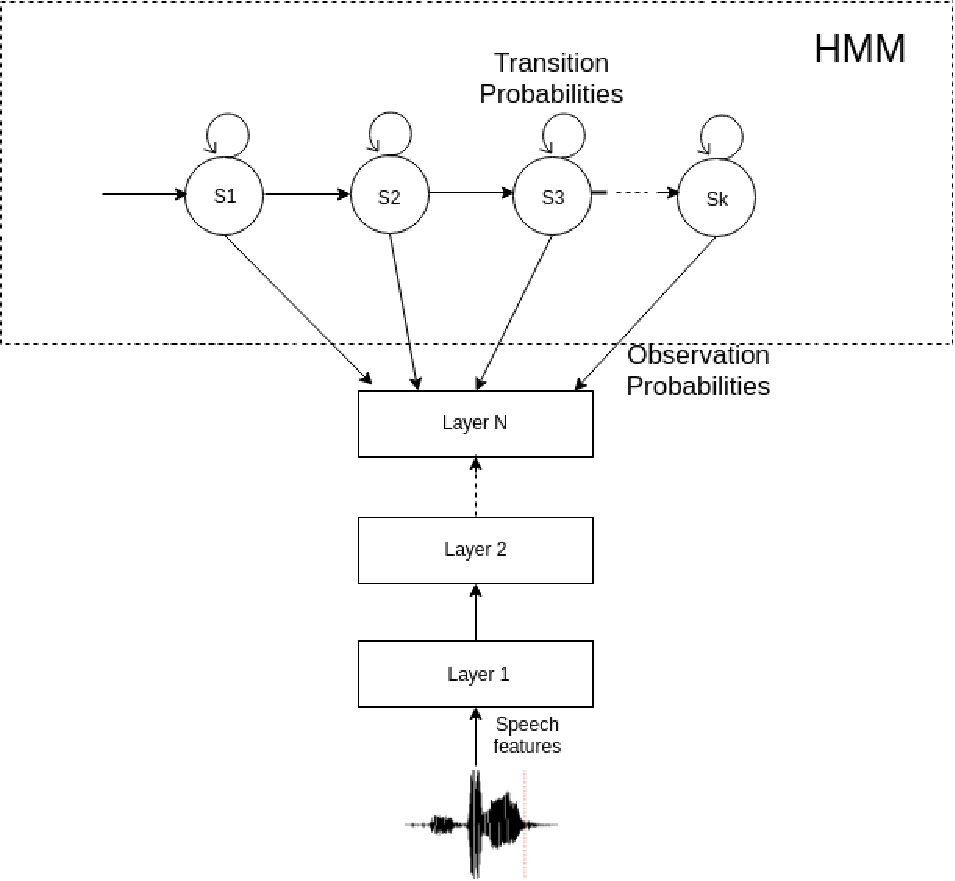
\includegraphics[width=13cm, height=7.5cm]{img/DNN-HMM.pdf}}
 \caption{DNN-HMM}
\label{fig:dnn}
\end{figure}
 
 
\subsection{Speech Decoding}
The most probable word sequences are detected by the speech HMM decoders which correspond to the words. Here we use various phoneme models typically triphone based model in AM. If a Language Model(LM) can be used for the decoding the performance getting much better. So decoding is also represented by making a search decision. After training the models in Kaldi we get some FST graph file that stores the Markov chain states with the weight of probability.\\
Nowadays word recognition is the most remarkable and successful form of ASR. Hidden Markov Model(HMM) which represents interword silence, connects the word.

  
\subsection{Speech Recognition Quality Evaluation}
Typically, WER is measured for calculating the accuracy of a speech recognizer. The minimum edit distance on words between the ASR output and reference transcription is computed for WER. Some edit operations such as substitution, deletion, insertion are used to minimize the edit distance as explains in \ref{wer} \\

\begin{equation} \label{wer}
    WEB=100*\frac{min\_dist(decoded_{AM,LM}(a),t,edit\_operation=\{Subs,Del,Ins\})}{\#\ words\ in\ t}
\end{equation}

As WER is an error function measuring the errors so the best case of WER = 0 for decoding. The WER value of 100 indicates that the decoding fails for every recognition of words in ASR.  

\end{document}